%http://tex.stackexchange.com/questions/100022/plotting-normal-distribution-in-pgfplots
\documentclass{article}
\usepackage{pgfplots}

\begin{document}

\pgfmathdeclarefunction{gauss}{3}{%
  \pgfmathparse{1/(#3*sqrt(2*pi))*exp(-((#1-#2)^2)/(2*#3^2))}%
}


\begin{tikzpicture}
\begin{axis}[
  no markers, 
  domain=0:6, 
  samples=100,
  ymin=0,
  axis lines*=left, 
  xlabel=$x$,
  every axis y label/.style={at=(current axis.above origin),anchor=south},
  every axis x label/.style={at=(current axis.right of origin),anchor=west},
  height=5cm, 
  width=12cm,
  xtick=\empty, 
  ytick=\empty,
  enlargelimits=false, 
  clip=false, 
  axis on top,
  grid = major,
  hide y axis
  ]

 \addplot [very thick,cyan!50!black] {gauss(x, 3, 1)};

\pgfmathsetmacro\valueA{gauss(1,3,1)}
\pgfmathsetmacro\valueB{gauss(2,3,1)}
\draw [gray] (axis cs:1,0) -- (axis cs:1,\valueA)
    (axis cs:5,0) -- (axis cs:5,\valueA);
\draw [gray] (axis cs:2,0) -- (axis cs:2,\valueB)
    (axis cs:4,0) -- (axis cs:4,\valueB);
\draw [yshift=1.4cm, latex-latex](axis cs:2, 0) -- node [fill=white] {$0.683$} (axis cs:4, 0);
\draw [yshift=0.3cm, latex-latex](axis cs:1, 0) -- node [fill=white] {$0.954$} (axis cs:5, 0);

\node[below] at (axis cs:1, 0)  {$\mu - 2\sigma$}; 
\node[below] at (axis cs:2, 0)  {$\mu - \sigma$}; 
\node[below] at (axis cs:3, 0)  {$\mu$}; 
\end{axis}

\end{tikzpicture}


\pgfmathdeclarefunction{gausss}{2}{%
  \pgfmathparse{1/(#2*sqrt(2*pi))*exp(-((x-#1)^2)/(2*#2^2))}%
}



\begin{tikzpicture}
\begin{axis}[
  no markers, domain=0:10, samples=100,
  axis lines*=left, xlabel=$x$, ylabel=$y$,
  every axis y label/.style={at=(current axis.above origin),anchor=south},
  every axis x label/.style={at=(current axis.right of origin),anchor=west},
  height=5cm, width=12cm,
  xtick={4,6.5}, ytick=\empty,
  enlargelimits=false, clip=false, axis on top,
  grid = major
  ]
  \addplot [fill=cyan!20, draw=none, domain=0:5.96] {gausss(6.5,1)} \closedcycle;
  \addplot [very thick,cyan!50!black] {gausss(4,1)};
  \addplot [very thick,cyan!50!black] {gausss(6.5,1)};


\draw [yshift=-0.6cm, latex-latex](axis cs:4,0) -- node [fill=white] {$1.96\sigma$} (axis cs:5.96,0);
\end{axis}

\end{tikzpicture}

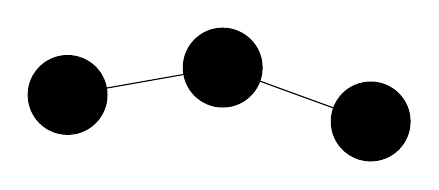
\begin{tikzpicture}
\draw[fill] (0,0) circle (.5) -- ++(10:2) circle (.5) -- ++(-20:2) circle (.5);
\end{tikzpicture}
\end{document}

http://tex.stackexchange.com/questions/106190/draw-a-chain-of-beads

%http://tex.stackexchange.com/questions/43610/plotting-bell-shaped-curve-in-tikz-pgf
